\section{Results}

\subsection{Sea ice experiment}

\begin{figure}[h!]
\centering
\caption{The evolution of the experiment from the left to the right, and from the top two images followed by the bottom.}
\label{experiment_evolution}
	\begin{subfigure}[t]{0.4\linewidth}
		\centering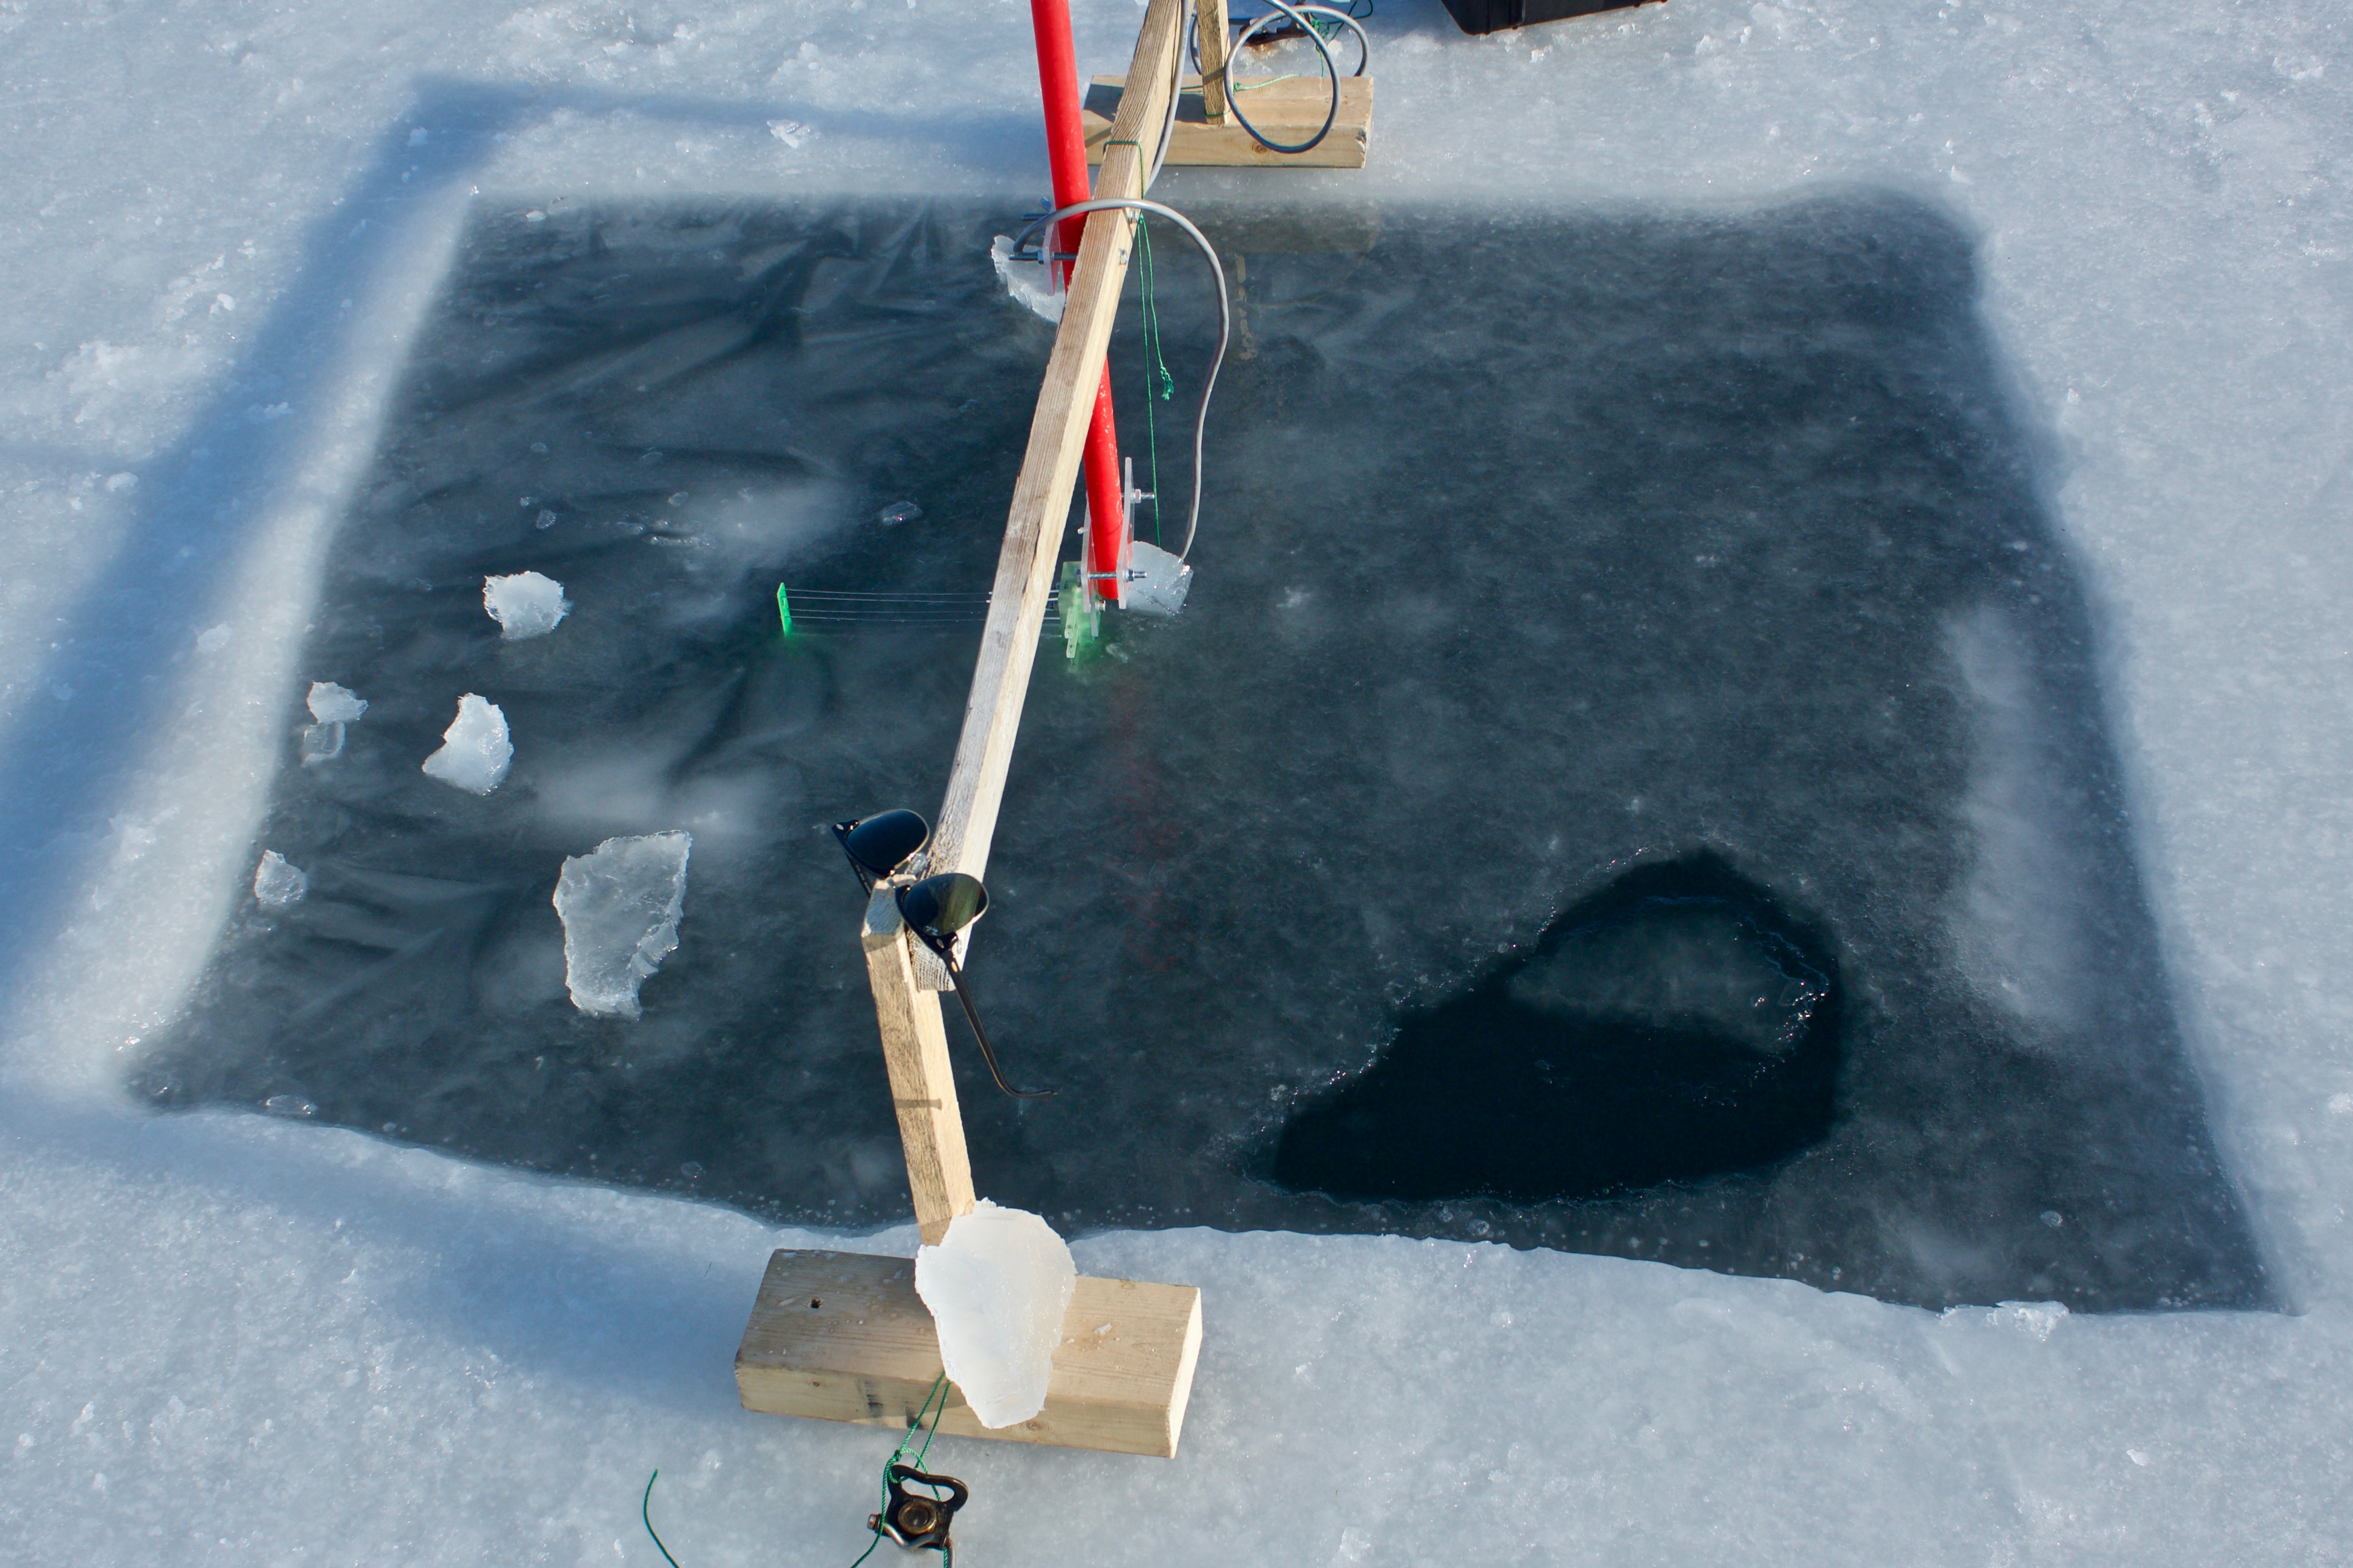
\includegraphics[width=0.8\linewidth]{_MG_6802}
		%\caption{(a)}
		%\label{stake_meas}
	\end{subfigure}
	\begin{subfigure}[t]{0.4\linewidth}
		\centering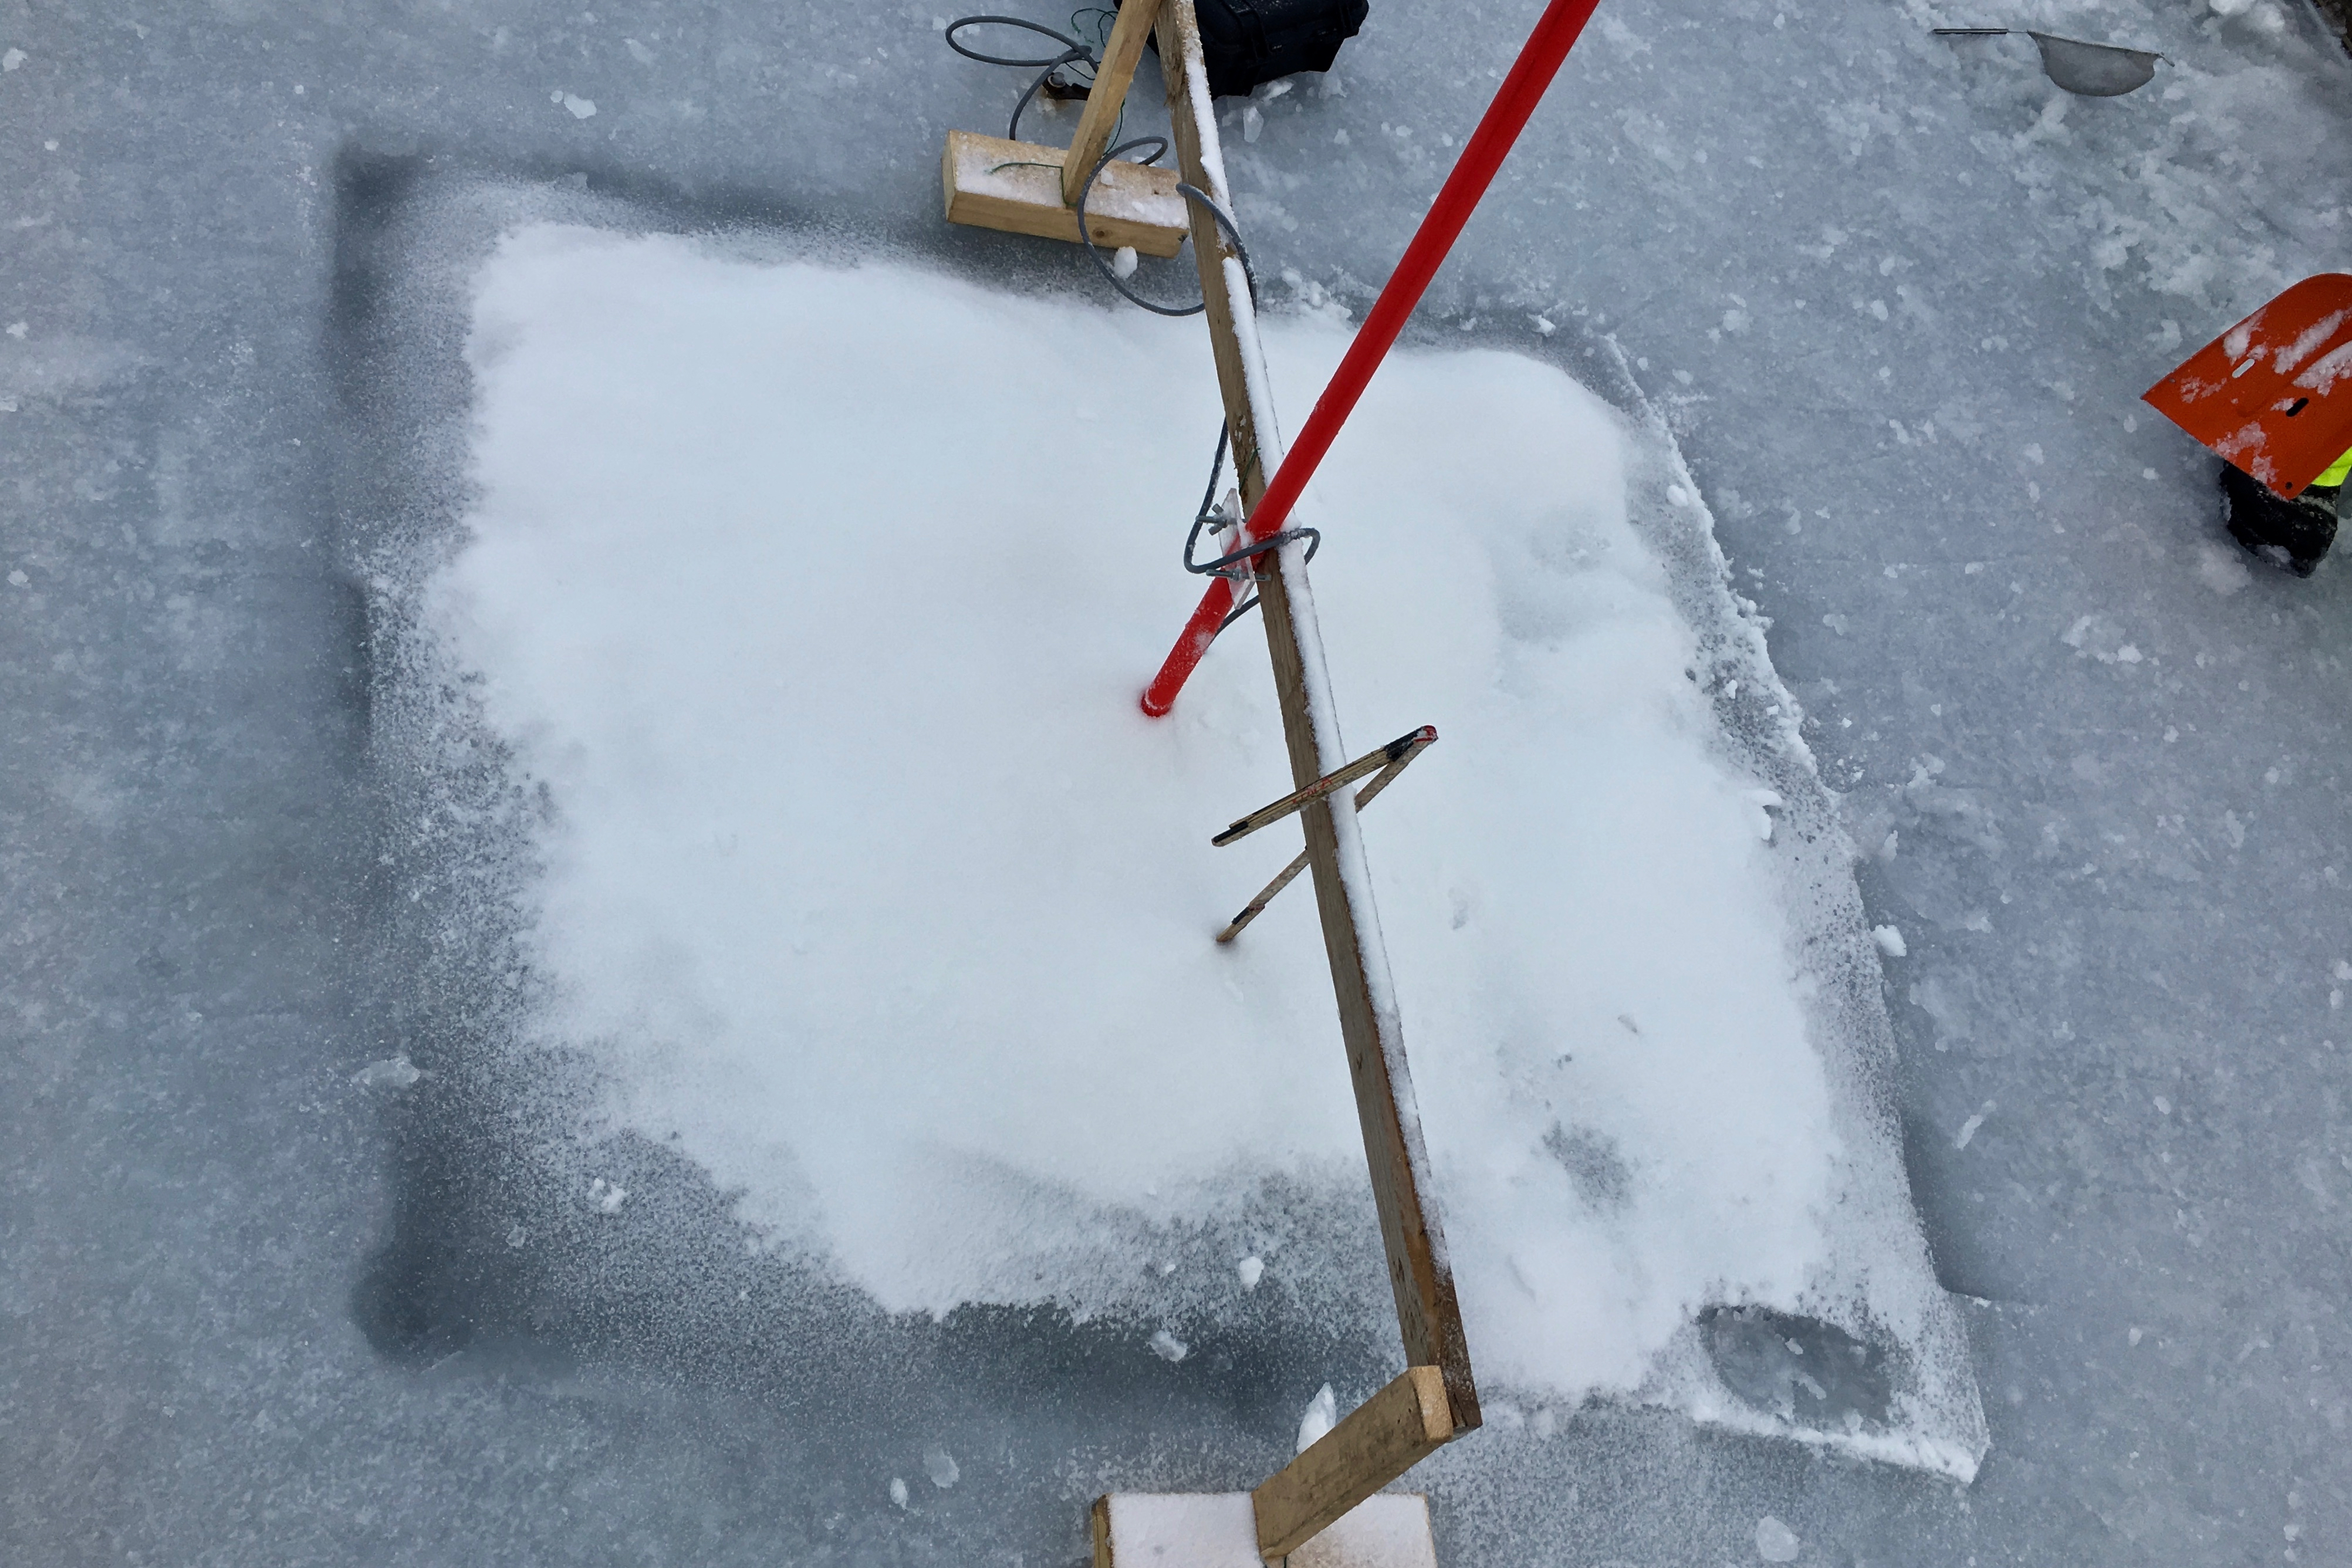
\includegraphics[width=0.8\linewidth]{IMG_0436}
		%\caption{(a)}
		%\label{stake_meas}
	\end{subfigure}
	\hfill
	%\medskip
	\begin{subfigure}[b]{0.4\linewidth}
		\centering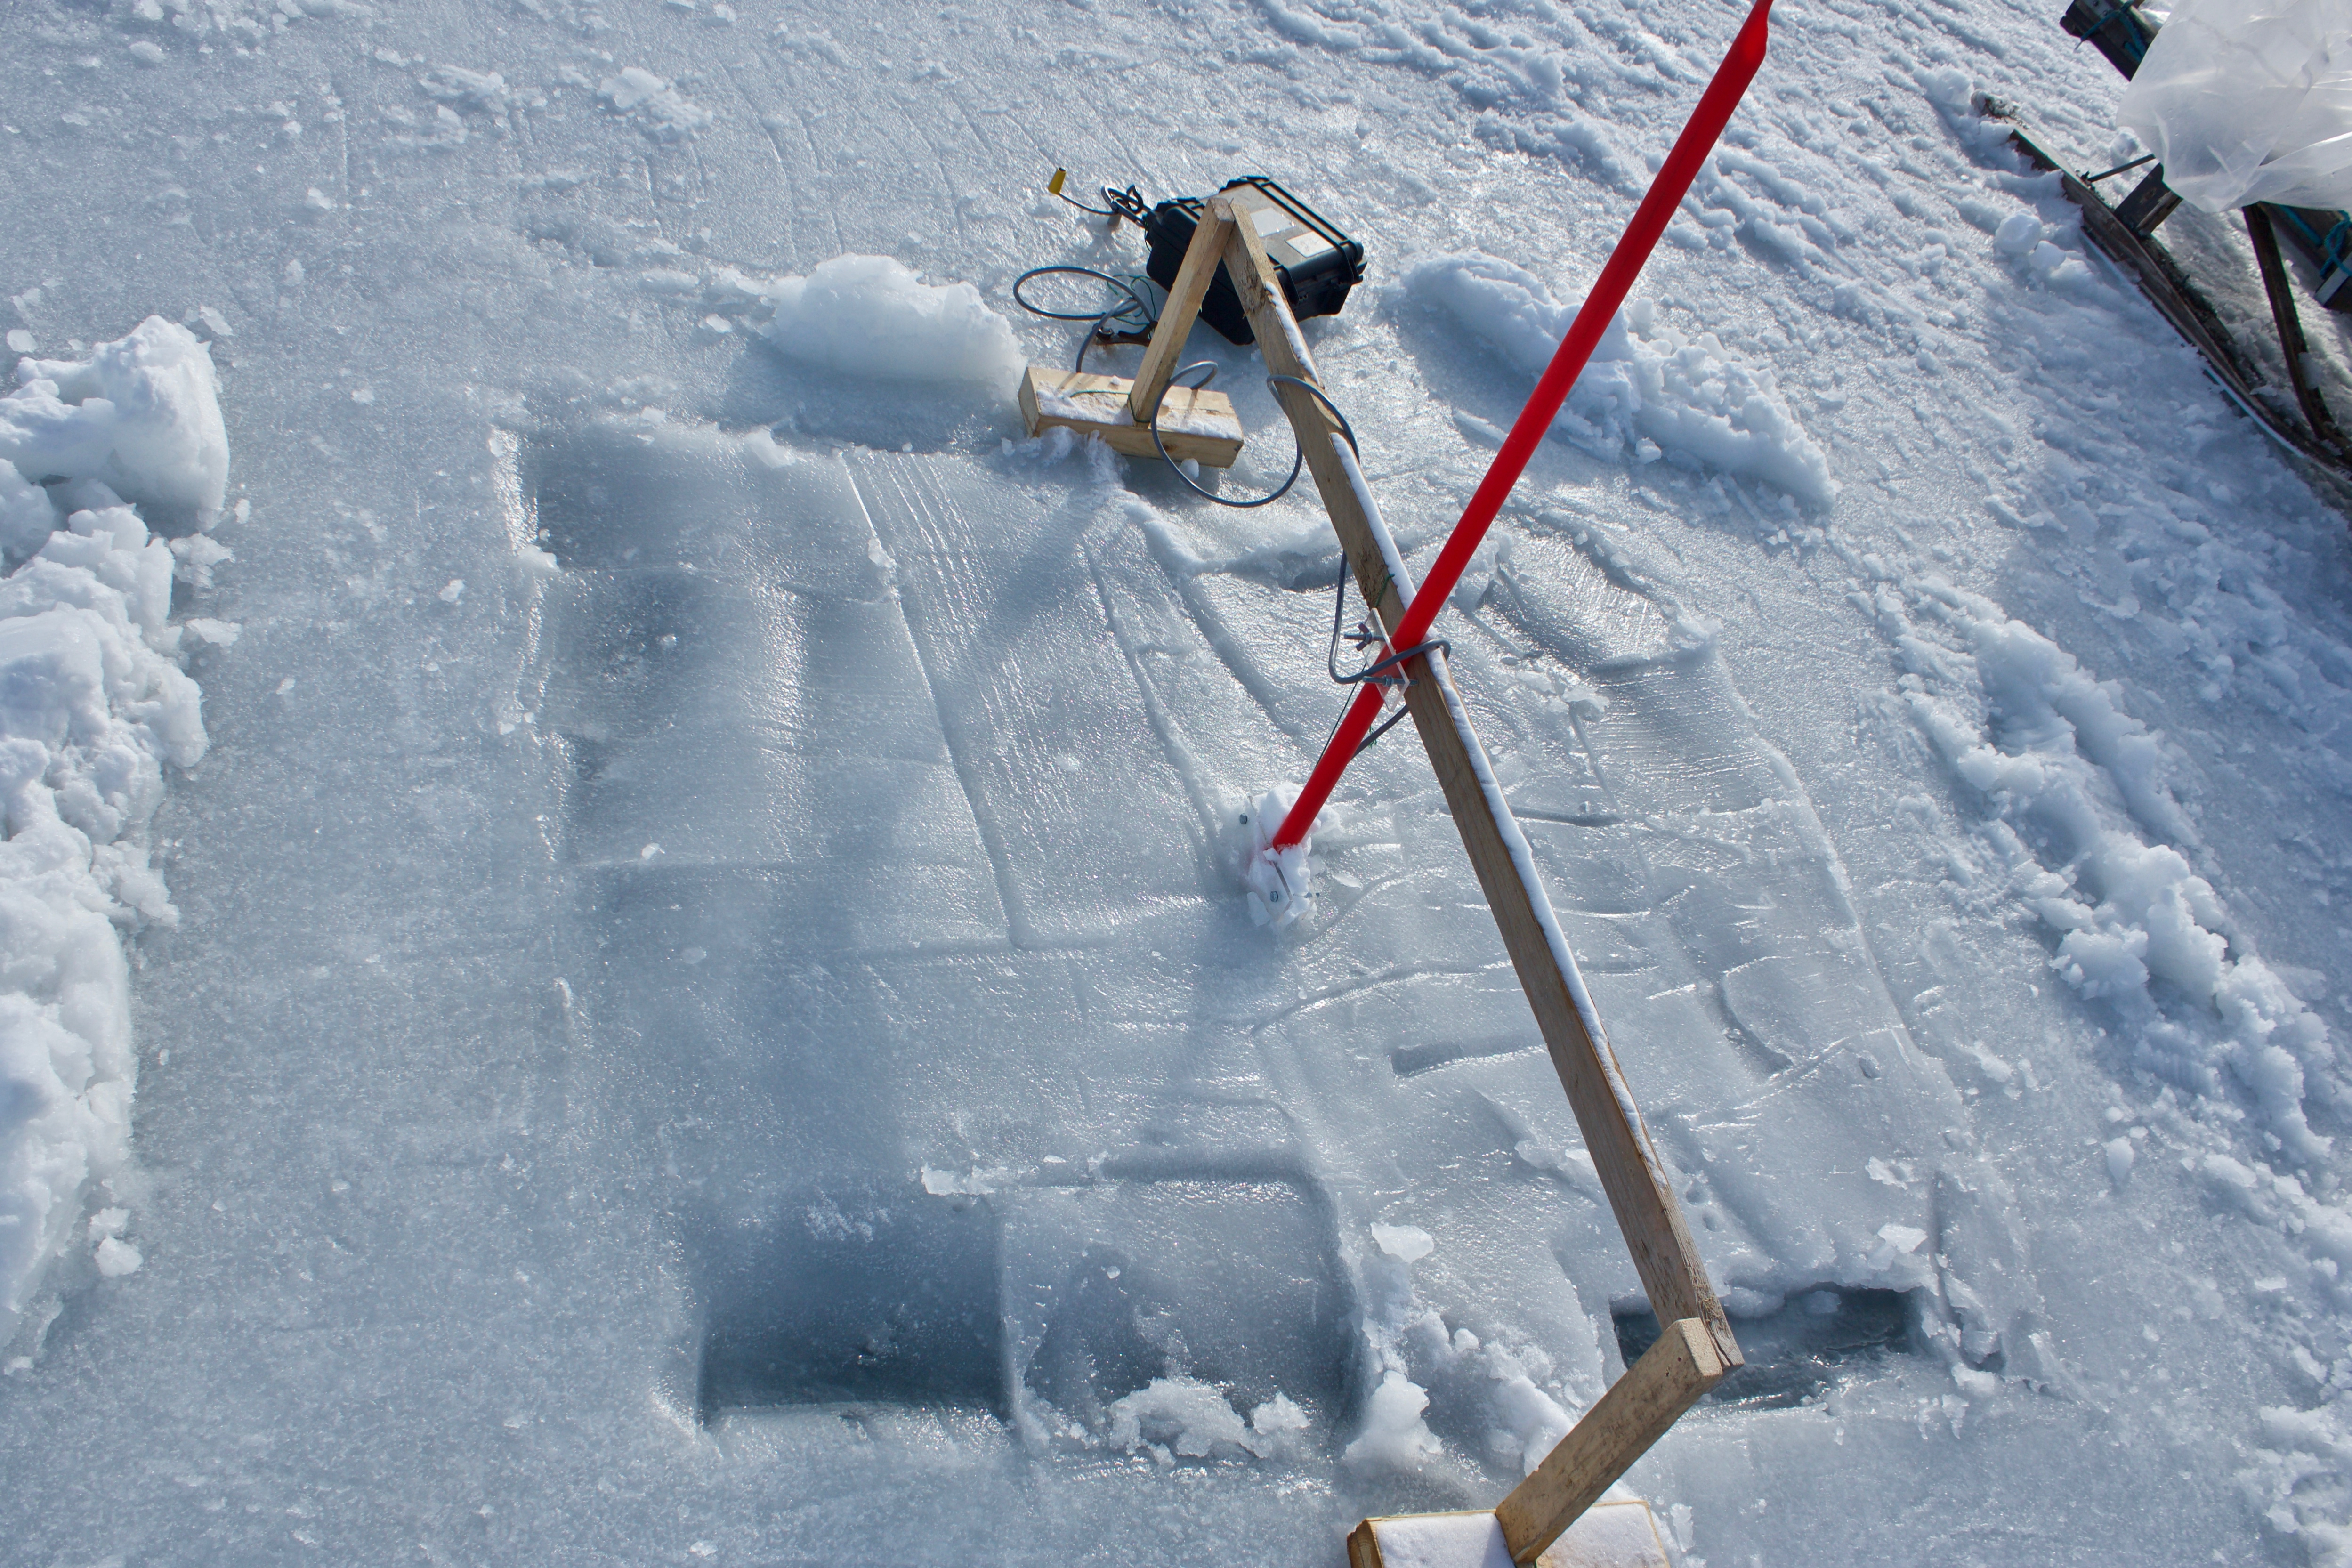
\includegraphics[width=0.8\linewidth]{_MG_6808}
		%\caption{(b)}
		%\label{probe_snow}
	\end{subfigure}
	\begin{subfigure}[b]{0.4\linewidth}
		\centering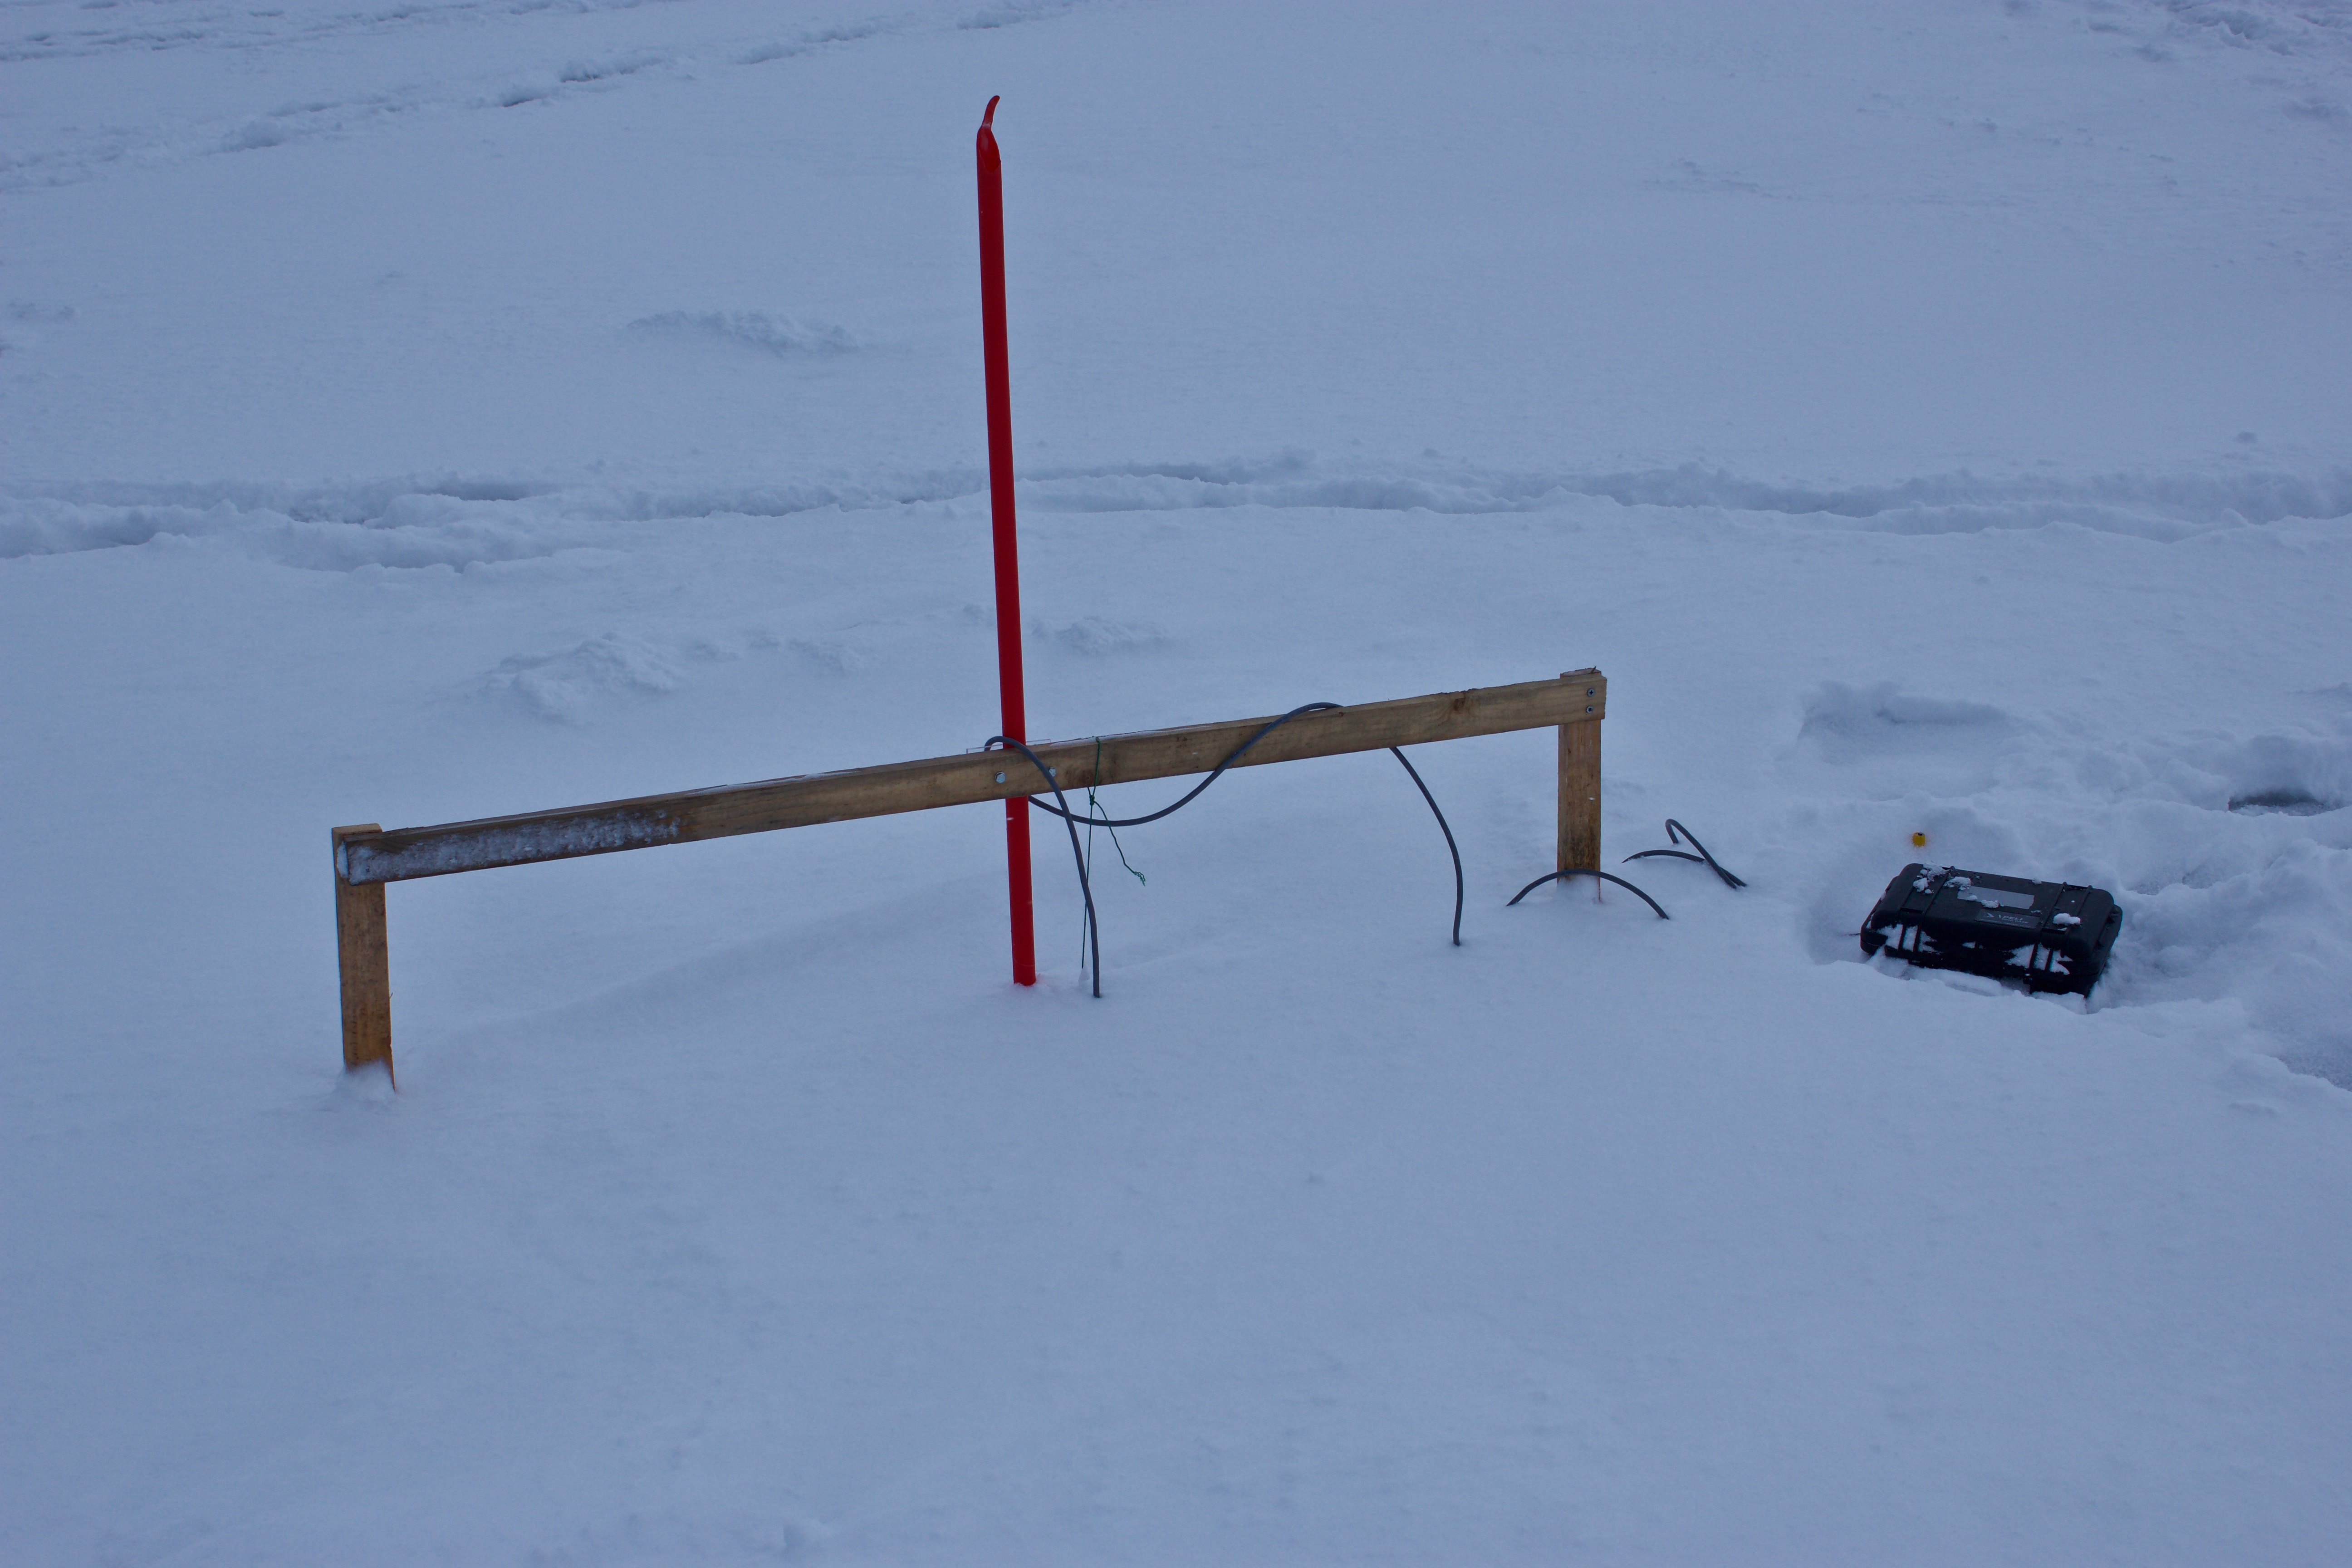
\includegraphics[width=0.8\linewidth]{_MG_6893}
		%\caption{(b)}
		%\label{probe_snow}
	\end{subfigure}
\end{figure}

The evolution of the snow experiment on the thin ice can be seen in \autoref{experiment_evolution}. The First image from top left, shows the newly grown sea ice the day after the experiment started. In this image it is hard not to notice the hole in the sea ice, which was first noticed at 14:20 on the 19. of April local time. The second top right image shows the state of the experiment after the snow was added. The third image at the bottom left shows the state of the experiment at 09:00 local time on the 20. of April. Here one can view the extensive amount of snow scraped of the day before. Take notice of how it is almost impossible to see where the original hole actual is. The final image at the bottom right shows the impact after a heavy snowfall that started on the 20. of April at around 12:00.\\ 
\\
At the end of the experiment an ice thickness of $8.6 \text{cm}\pm 0.002 \text{cm}$ was measured with a vernier caliper. Only two of the six wires in the ocean was frozen into the ice. The ice was measured to be $0.3 \text{cm}\pm 0.2 \text{cm}$ from the third wire pair down, counted from the surface. The results from sawed of ice piece from the newly grown sea ice is presented in Table \autoref{Ice_core}.

\begin{table}[h!]
\centering
\caption{Data from the ice cores that was taken for comparison}
\label{Ice_core}
\begin{tabular}{ccc}
\multicolumn{3}{c}{Harp 2 Ice "core" data}                      \\
Depth {[}cm{]} & Temperature {[}$\deg$C{]} & Salinity {[}PSU{]} \\ \hline
0-2.5          & -1.9                      & 9.4                \\
2.5-7          & -1.8                      & 9.4                \\
\end{tabular}
\end{table}

\subsubsection{Temperature}
\begin{figure}[h!]
	\centering
	\includegraphics[width=0.9\textwidth]{temperature_harp2}
	\caption{The temperature evolution of the sea ice experiment plotted as a function of depth. The black horizontal line represents the surface, the vertical black dotted lines marks the day change, and the vertical white dotted line marks the beginning of the second phase of the experiment. Each grid cell represents 6 hours of data recording.}
	\label{temperatureharp2}
\end{figure}

\autoref{temperatureharp2} shows the interpolated temperature evolution as a function of depth. The black line represents the surface, the white vertical dotted line represents where the beginning of the second phase of the experiment, and the black vertical dotted lines marks the day change. The overall trend is that the temperature increases with depth, except for the time period 06:00-12:00 on the 19. of April. The coldest and the hottest recorded temperatures was measured by the temperature sensors highest up. $-12.3 \deg C \pm 0.15$, and $3 \deg C \pm 0.15$ respectively. Other than that, it can clearly be seen that the strongest temperature changes occur in the beginning of the experiment, when there is the largest temperature difference between the top sensor and the bottom sensor. Also, it can be seen that the entire column has almost the same temperature from the white line until the end of the experiment, at around $-2 \deg C$. Furthermore, some spikes in the temperature with varying magnitude and length can be seen just before 12:00 every day at the sensors on the bottom. 



\subsubsection{Bulk Salinity}
\begin{figure}[h!]
	\centering
	\includegraphics[width=0.9\textwidth]{Bulk_salinity_harp2}
	\caption{The salinity evolution of the sea ice experiment plotted as a function of depth. The black horizontal line represents the surface, the vertical black dotted lines marks the day change, and the vertical white dotted line marks the beginning of the second phase of the experiment. Each grid cell represents 6 hours of data recording.}
	\label{salinityharp2}
\end{figure}

\autoref{salinityharp2} shows the interpolated salinity evolution as a function of depth. The black line represents the surface, the white vertical dotted line represents where the beginning of the second phase of the experiment, and the black vertical dotted lines marks the day change. 

The overall trend is that the salinity decreases over time, and also in in parts as a function of depth. The highest recorded salinity values was recorded at the sensors closest too the surface in the beginning of the experiment, and the sensor at the top after the white dotted line. The sensors recorded a salinity of $50 \text{g}/\text{kg} \pm 1.76\text{g}/\text{kg}$, and $104 \text{g}/\text{kg} \pm 1.76\text{g}/\text{kg}$ respectively. The lowest recorded salinity values was in the majority of the time recorded at the sensor that was at $-2$ cm depth. The lowest value that this sensor recorded was a salinity of $5 \text{g}/\text{kg} \pm 1.76\text{g}/\text{kg}$. The lowest value recorded overall was recorded at the sensor at $-6$ cm depth, and it recorded a salinity of $4.2\text{g}/\text{kg} \pm 1.76\text{g}/\text{kg}$ at just before 12:00 UTC on the 19. of April.

Other than that it can clearly be seen that the strongest salinity changes take place at the beginning of the experiment, and after the white dotted line on the two sensors highest up. It can also be seen that there is some very distinct layering of the salinity values at the four lowest sensors. Another notable layer is the one after the white dotted line at just above $-4$ cm depth. Furthermore, some interesting changes are occurring periodically at the bottom sensors, usually over a period of 12 hours. 



\subsubsection{Liquid Fraction}
\begin{figure}[h!]
	\centering
	\includegraphics[width=0.9\textwidth]{Liquid_fraction_harp2}
	\caption{The liquid mass fraction evolution of the sea ice experiment plotted as a function of depth. The black horizontal line represents the surface, the black dotted lines marks the day change, and the white dotted line marks the beginning of the second phase of the experiment. Each grid cell represents 6 hours of data recording.}
	\label{liquidfractionharp2}
\end{figure}

\autoref{liquidfractionharp2} shows the interpolated liquid mass fraction evolution as a function of depth. The black line represents the surface, the white vertical dotted line represents where the beginning of the second phase of the experiment, and the black vertical dotted lines marks the day change. 

A liquid mass fraction value of one indicate that everything is liquid (all black), and a liquid mass fraction value of zero indicate that everything is solid (all white). The highest liquid mass fraction value recorded was $0.9$ at $-10$cm depth during almost the whole experiment, as the value only changed with $\pm 0.01$ from $0.9$ throughout the experiment. The lowest liquid mass fraction value recorded was $0.23$ at the surface sensor at 09:30 UTC on the 21. of April. 

In the range of 4 cm above and below the surface it can be seen that the liquid mass fraction decreases over time, and also in general as a function of depth. In this depth range there is also a sudden increase in the liquid mass fraction just before 12:00 on the 19. of April, after which the liquid mass fraction decreases back to what it was before the sudden increase. Below the depth of $-6$cm, a layer of increased liquid mass fraction can be seen with a sudden increase at the same time as the one mentioned above. Other than that, the liquid mass fraction stays very stable, and there is no large changes in its value. 


\subsection{Snow ice experiment}


\autoref{liquidfractionsnow} shows the brine percolation through the snow, and then refreezing at the lower wires. The bottom wire was the first to experience the rise of water and was fully immersed after just a couple of hours, there is some percolation up to $8 cm$ around the same time, and the wires under 6 cm had a water content of over $0.45$. After the snowfall at 12h UTC, 20.04.18. The percolation was accelerated, and over $0.6$ of the wires, where covered in brine after 12 hours.

\begin{figure}[h!]
	\centering
	\includegraphics[width=0.9\textwidth]{Water_content}
	\caption{The liquid volume fraction in the snow plotted as a function of time
    and heights of wires, data between wires is interpolated.}
	\label{liquidfractionsnow}
\end{figure}

%There is a nice gradient at towards the end, where it is possible to see how the ocean heat flux propagates through the ice. The two previous AGF-211 Cruises has also proven that snow has an isolating effect.




%------
%'Exeeds Standard' criteria for Report Grading:
%The Results presents the most important and representative data in clear, well-labelled figures and tables. Results are thorough, original, and easy to interpret.
%------